\chapter{Background}
\label{chapter2}
In this chapter, we discuss the background knowledge and introduce notation that will be used for the thesis. We begin with intruding graphical models formally, which is followed with the inference tasks of graphical models. We also discusses the learning principles in model learning. \textcolor{blue}{Provide more thorough explanation here after this chapter is finished}.

\section{Graphical Models}
Graphical models provide a formal graph representation of statistical dependency of complex problems. The conditional independence of any random variables can be conveniently analyzed in a graphical model (I-map, d-Separation, markov blanket). More importantly, a intractable complex problem can be resolved by local interactions of small parts of a graphical model.

More formally, a graphical model is a representation of a collection of random variables (along their domains) and nonnegative functions. Let $\bm{X}= (X_1, X_2, \cdots, X_N)$ be a vector of random variables, where an element variable $X_i$ can be either discrete or continuous and takes values from its domain $\Xx_i$. Note that domain of a random variable is not necessary be the same as that of another.

We use lower case letters, e.g. $x_i \in \Xx_i$, to indicate a value assignment of $X_i$. Similarly, $\bm{x}$ denotes the assignment of $\bm{X}$, and $  p(x_1, x_2, \cdots, x_N) = p(X_1 = x_1, X_2 = x_2, \cdots, X_N = x_N)$,
which sometimes is simplified as $p(\bm{x})=p(\bm{X}=\bm{x})$. We denote $\bm{\Xx} = \prod_{x=1}^{N} \Xx_i$ and then $\bm{x}\in \bm{\Xx}$.

As mentioned in Chapter~\ref{section1.1}, a graphical model can be directed or undirected. Directed graphical model also is also know as Bayesian network or generative model in literature \cite[Chapter~8]{Bishop:2006:PRM:1162264}. We might use the names alternatively.
A graphical model over random variable $\bm{X}$ consists of a set of local nonnegation functions.

In directed graphical models, i.e. Bayesian networks, the local functions are conditional probability function. The joint probability distribution is represented as product of these conditional probability functions,
\begin{equation}
  p(\bm{x}) = \prod_{n=1}^{N}p(x_n| \Pp(x_n)),
\end{equation}
where $\Pp(\cdot)$ denotes the set of parent nodes in the directed graph. In an directed graphical model, the local functions are actually conditional probability distributions, e.g. $\{p(X_n| \Pp(X_n))\}$, which are properly normalized and sum to one. Additionally, sampling from a underlining distribution $p(\bm{X})$ of a directed graphical model is efficient. Due to acyclic property of directed graph, by the well know \textit{ancestral sampling}, a sample $\{x_1, x_2, \cdots, x_N\}$ can be drawn sequentially via following the directed edges. In another word, $x_n$ is always sampled after $\Pp(x_n)$. This process might be viewed as the 'generative' process of signal $\bm{x}$.

A Bayesian network is usually easier to be interpreted due to the fact that the its local functions are conditional probabilities. But Bayesian networks can only to applied to limited cases where influence between variables is directional. In many practical cases, interaction between variables can not be naturally described by impact with directionality. Problems of this kind can be represented by undirected graphical models, i.e. Markov random field (MRF). Under certain condition, a Bayesian network can be perfectly represented by a Markov random field without loss of independence information by moralizing edges \cite[Chapter~4.5]{koller2009pgm}. Instead of conditional probability, the local functions of MRF represents the compatibility of states of different variables, which are known as potential factors in literature. Different from conditional probabilities the Bayesian network, the potential factors in MRFs are not necessary summed to one. We provide a toy example of MRF with three variable nodes as follows.
\begin{figure}[!t]
  % \captionsetup[subfigure]{justification=centering}
  \begin{subfigure}{.3\textwidth}
    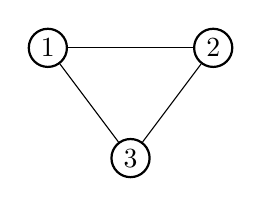
\begin{tikzpicture}
      \begin{scope}[scale=0.7]
        \tikzstyle{cnode} = [thick, draw=black, circle, inner sep = 2pt,  align=center]
        \node[cnode] (x1) at (0,0) {$1$};
        \node[cnode] (x2) at (3,0) {$2$};
        \node[cnode] (x3) at (1.5,-2) {$3$};
        \draw[-] (x1) -- (x2);
        \draw[-] (x1) -- (x3);
        \draw[-] (x2) -- (x3);
      \end{scope}
    \end{tikzpicture}
  \end{subfigure}
  \begin{subfigure}{0.3\textwidth}
    \begin{tabular}{llc}
      \toprule
      $X_1$ & $X_2$ & $\phi(X_1, X_2)$ \\
      \midrule
      0  &  0  &  10 \\
      0  &  1  &  1 \\
      1  &  0  &  1 \\
      1  &  1  &  10\\
      \bottomrule
    \end{tabular}
  \end{subfigure}
  \begin{subfigure}{0.05\textwidth}
    \centering
    \begin{tikzpicture}
      \node[] at (0,0) {$\cdots$};
    \end{tikzpicture}
  \end{subfigure}
  \begin{subfigure}{0.3\textwidth}
    \begin{tabular}{llc}
      \toprule
      $X_2$ & $X_3$ & $\phi(X_1, X_2)$ \\
      \midrule
      0  &  0  &  5 \\
      0  &  1  &  3 \\
      1  &  0  &  3 \\
      1  &  1  &  5 \\
      \bottomrule
    \end{tabular}
  \end{subfigure}
  \caption{A Markov random field with three binary nodes. Potential factors are represented by tables.}
  \label{chp2:fig:toy_mrf}
  \hspace{1cm}
\end{figure}

\begin{example}\label{chpt2:mrf-3node-example}
  As shown in Figure~\ref{chp2:fig:toy_mrf}, the MRF encodes dependency of three random variables $X_1$, $X_2$, and $X_3$, where node $i$ is associated with variable $X_i$ and each has a binary domain, i.e. $\Xx_i = {0,1}$ for $i =1,2,3$. Three potential factors of the MRF together define the joint distribution
  \begin{equation*}
    p(\bm{x}) = \frac{1}{Z} \phi_{1,2}(x_1, x_2) \phi_{2,3}(x_2, x_3) \phi_{1,3}(x_1, x_3)
  \end{equation*}
  where $Z = \sum_{x_1, x_2, x_3}\phi_{1,2}(x_1, x_2) \phi_{2,3}(x_2, x_3) \phi_{1,3}(x_1, x_3)$ normalizes the potential factors such that $p(\bm{x})$ sums to one. The exemplified potential factors in Figure~\ref{chp2:fig:toy_mrf} demonstrate that it is more compatible or likely when $X_1$, $X_2$ and $X_3$ are in the same state (either $0$ or $1$) than they are configured into different states.
\end{example}

From the above example to a formal statement, a MRF over random vector $\bm{X}$ can be represented by a undirected graph $\Gg(\Vv, \Ee)$, with each node $i \in \Vv$ is associated with a random variable $X_i$ and undirected edge set $\Ee \subset \Vv \times \Vv$. This MRF encodes a collection of distributions that factorize as
\begin{equation}\label{chp2:eq:mrf-definition}
  p(\bm{x};\bm{\theta}) = \frac{1}{Z(\bm{\theta})} \prod_{\alpha \in \Ii} \phi_{\alpha}(\bm{x_{\alpha}};\bm{\theta}),
\end{equation}
where $\Ii$ is the set of indexes of potential factors, and each factor $\phi_{\alpha}$ for $\alpha\in \Ii$ is defined on subset of $\bm{X}$, i.e. $\phi_{\alpha}: \Xx_{\alpha} \rightarrow \RR^{+} \cup \{0\}$, where $\Xx_{\alpha} = \prod_{i\in \alpha}\Xx_i$ is the domain of potential factor $\phi_{\alpha}$. The scope of factor $\alpha$ is $\bm{X}_{\alpha} = \left\{ X_i| i\in \alpha \right\}$. In \eqref{chp2:eq:mrf-definition},
\begin{equation}
  Z(\bm{\theta}) = \sum_{\bm{x}} \prod_{\alpha \in \Ii} \phi_{\alpha}(\bm{x_{\alpha}};\bm{\theta})
\end{equation}
is the \textit{partition function}. Apparently, the partition function normalizes the potential factors such that $p(\bm{x}; \bm{\theta})$ is a proper probability.

\begin{remark}
  We can compare directed and undirected graphical models with regarding the following aspects.
  \begin{itemize}
  \item \textit{Representation}: The structure and the parameters directed graphical models provide a natural representation for many types of real-world domains. MRF representation is not usually as intuitive as directed graphical models. But the acyclic property of directed graphical models also limits their representation power. On the other hand, MRFs can be either cyclic or acyclic, which offers the flexibility of graph structure and can simplify the graphical representation. Due to the requirement is weaker for potential factors than that for conditional distribution, the representation of MRFs are richer. 
  \item \textit{Local nonnegative functions}: The local functions are conditional probability functions in directed graphical models, but are potential factors (nonnegative) in undirected cases.
  \item \textit{Sampling}: Sampling is more straightforward within generative models (directed) than that in MRFs.
  \item \textit{Normalization}: Since each local function is a conditional probability function in directed graphical models, partition function for normalization is not needed. A MRF in general comes with partition functions, since the requirement on potential factors are weaker than a conditional probability distribution.
  \end{itemize}
\end{remark}




\subsection{Alternative Representation of MRF}
\begin{figure}[!t]
  % \captionsetup[subfigure]{justification=centering}
  \begin{subfigure}{.5\textwidth}
    \centering
    \begin{tikzpicture}
      \begin{scope}[scale=0.7]
        \tikzstyle{cnode} = [thick, draw=black, circle, inner sep = 2pt,  align=center]
        \tikzstyle{nnode} = [thick, rectangle, rounded corners = 0pt,draw,inner sep = 5pt]
        \node[cnode] (x1) at (0,0) {$1$};
        \node[above=0.2mm of x1] {$X_1$};
        \node[cnode] (x2) at (3,0) {$2$};
        \node[above=0.2mm of x2] {$X_2$};
        \node[cnode] (x3) at (1.5,-2) {$3$};
        \node[below=0.2mm of x3] {$X_3$};

        \node[nnode] (f12) at (1.5, 0) {};
        \node[] at ($(f12) + (0,0.6)$) {$\phi_{1,2}$};
        \node[nnode] (f13) at (0.75, -1) {};
        \node[] at ($(f13) + (-0.8,0)$) {$\phi_{1,3}$};
        \node[nnode] (f23) at (2.25, -1) {};
        \node[] at ($(f23) + (0.80,0)$) {$\phi_{2,3}$};
        \path[-, draw, thick]
        (x1) edge node {} (f12)
        (f12) edge node {} (x2)
        (x2) edge node {} (f23)
        (f23) edge node {} (x3)
        (x3) edge node {} (f13)
        (f13) edge node {} (x1)
        ;
      \end{scope}
      
    \end{tikzpicture}
    \caption{Factor graph representation.}
    \label{chpt2:fig:factor-graph-3node-example}
  \end{subfigure}
  \begin{subfigure}{.5\textwidth}
    \centering
    \begin{tikzpicture}
      \begin{scope}[scale=0.7]
        \tikzstyle{cnode} = [thick, draw=black, circle, inner sep = 2pt,  align=center]
        \tikzstyle{cfnode} = [thick, draw=black, fill=gray,circle, inner sep = 2pt,  align=center]
        \tikzstyle{nnode} = [thick, rectangle, rounded corners = 0pt,draw,inner sep = 5pt]
        \node[cnode] (x1) at (0,0) {$1$};
        \node[above=0.2mm of x1] {$X_1$};
        \node[cfnode] (x2) at (3,0) {$2$};
        \node[above right=0.2mm and 0.2mm of x2] {$X_2=x_2$};
        \node[cnode] (x3) at (1.5,-2) {$3$};
        \node[below=0.2mm of x3] {$X_3$};
        \node[nnode] (f12) at (1.5, 0) {};
        \node[] at ($(f12) + (0.2,0.6)$) {$\phi_{1,2}\bm{1}(x_2)$};
        \node[nnode] (f13) at (0.75, -1) {};
        \node[] at ($(f13) + (-0.8,0)$) {$\phi_{1,3}$};
        \node[nnode] (f23) at (2.25, -1) {};
        \node[] at ($(f23) + (1.50,0)$) {$\phi_{2,3}\bm{1}(x_2)$};
        \path[-, draw, thick]
        (x1) edge node {} (f12)
        (f12) edge node {} (x2)
        (x2) edge node {} (f23)
        (f23) edge node {} (x3)
        (x3) edge node {} (f13)
        (f13) edge node {} (x1)
        ;
      \end{scope}
    \end{tikzpicture}
    \caption{Conditioning on $X_2=x_2$}
    \label{chpt2:fig:factor-graph-3node-example-condition}
  \end{subfigure}

  \caption{A Markov random field is represented by a factor graph, i.e. \ref{chpt2:fig:factor-graph-3node-example}, and conditioning of the Markov random field \ref{chpt2:fig:factor-graph-3node-example-condition}.}
  \label{chp2:tab:toy-factor-graph}
  \hspace{1cm}
\end{figure}

The representation of a MRF by $\Gg(\Vv, \Ee)$ as explained above is compact, but the potential factors are missing. An alternative representation of MRF is \textit{factor graph} \cite{kschischang2001factor_graph},
which is a bipartite graph topology. In a factor graph, a potential factor is explicitly represented as a factor node, as counterpart of variable node associated with a random variable.
\begin{definition}\label{chpt2:def:factor-graph}
  A factor graph $\Gg_F$, is a bipartite graph that represents the factorization structure of \eqref{chp2:eq:mrf-definition}. A factor graph has two types of nodes: i) a variable node for each variable $x_i$; ii) a factor node for each potential function $\phi_{\alpha}$. An edge between a variable node $i$ and factor node $\alpha$ if and only if $x_i$ is argument of $\phi_{\alpha}$. We would denote a factor graph by $\Gg_F(\Vv \cup \Ff, \Ee_F)$ with $\Vv$ as the set of variable nodes, $\Ff$ as the set of factor nodes, and $\Ee_F$ the set of undirected edges.
\end{definition}
\begin{example}
  Let us represent the Example~\ref{chpt2:fig:factor-graph-3node-example} by a factor graph, which is shown in Figure~\ref{chpt2:fig:factor-graph-3node-example}. Different from the representation by $\Gg(\Vv, \Ee)$ in Figure~\ref{chp2:fig:toy_mrf}, factor nodes are explicitly represented by square nodes.
\end{example}


\subsection{Conditioning on Observations in MRFs}
It is not rare that a graphical model may contain observed variable. The node set of a MRF can be separated into a subset $\Vv_O$ of nodes, that are associated with observed variable $\bm{X}_O$, and a subset $\Vv_U$ of nodes associated with unobserved variable $\bm{X}_U$. For an observation $\bm{X}_O=\bm{x}_O$,
\begin{equation}
  p(\bm{x}_U|\bm{x}_O;\bm{\theta}) = \frac{p(\bm{x}; \bm{\theta})}{p(\bm{x}_O;\bm{\theta})} =  \frac{Z(\bm{x}_O,\bm{\theta})}{Z(\bm{\theta})},
\end{equation}
where 
\begin{align}
  \tilde{p}(\bm{x}; \bm{\theta}) &= \prod_{\alpha \in \Ii} \phi_{\alpha}(\bm{x}_{\alpha};\bm{\theta}), \nonumber \\
  Z(\bm{x}_O, \bm{\theta}) &= \sum_{\bm{x}_U} \tilde{p}(\bm{x}; \bm{\theta}), \nonumber \\
  Z(\bm{\theta}) &= \sum_{\bm{x}_O}\sum_{\bm{x}_U} \tilde{p}(\bm{x}; \bm{\theta}).
\end{align}
This means that a condition probability can be computed by partition function and sub-partition functions. Alternatively, the conditional probability can be written as
\begin{equation}
  p(\bm{x}_U|\bm{x}_O;\bm{\theta}) = \frac{\tilde{p}(\bm{x}; \bm{\theta})\bm{1}(\bm{x}_O)}{\sum_{\bm{x}_U}\tilde{p}(\bm{x}; \bm{\theta})\bm{1}(\bm{x}_O)}
\end{equation}

where $\bm{1}(\bm{x}_O)$ is an indicator function and equals to one if and only if the states of nodes in $\Vv_O$ are jointly $\bm{x}_O$. This can be understood as clamping nodes in $\Vv_O$ of the MRF to configuration $\bm{x}_O$, i.e. the domain of $\bm{X}_O$ becomes a set containing only $\bm{x}_O$. (For instance, an example of conditioning on a variable node is shown in Figure~\ref{chpt2:fig:factor-graph-3node-example-condition}.) Then any inference applicable to a MRF applies to the MRF with nodes clamped as well.

In addition to the above intuitions, conditioning can also be understood as a process of reducing the graph of a MRF. When a MRF is conditioned on $\bm{x}_O$, the variables nodes of set $\Vv_O$ are removed from $\Gg$, along with their edges. The potential factors with regarding to $\Vv_U$ are modified accordingly \cite[Chapter~4.2.3]{koller2009pgm}.

It can be seen that MRF framework is capable to handle conditioning as well. Therefore, in the following part of the thesis, it might or might not have bee based on conditioning observed variables when a MRF is mentioned.

\section{Divergence}\label{chpt2:sec:devergence}
Before we get into more discussion about inference and learning topics, we firstly introduce the concept of \textit{divergence} measures since principles of both learning and inference are closed related with divergence measure.
A divergence measure play a fundamental role when we try to use a probability density (or mass for discrete cases) function $q$ to approximate another probability density function $p$. A divergence measure is used to formal quantity how much information is lost when $p$ is represented by $q$. Denote $\PP$ as the space of measures $p$ and $q$, i.e. $p, q \in \PP$.
\begin{definition}
  Given the space of probability density (or mass) function $\PP$ for a random variable $\bm{x}$, a divergence on this space is defined as a function $D(p\|q): \PP \times \PP \rightarrow \RR$ such that $D(p\|q) \geq 0$ for all $p, q \in \PP$ and $D(p\|q)=0$ if and only if $p=q$.
\end{definition}

Here we introduce the classic \textit{Kullback-Leibler divergence} \cite{kullback1959, kullback1951}, KL divergence for short, which is one of the most widely used divergence measures in machine learning, statistics and information theory.
\begin{definition}
  The Kullback-Leibler (KL) divergence on $\PP$ is defined as a function $KL(\cdot \| \cdot): \PP \times \PP \rightarrow \RR^{+} \cup {0}$ with the following form
  \begin{equation}\label{chpt2:def:kl-divergence}
    \mathrm{KL}(p\|q) = \sum_{\bm{x}}p(\bm{x}) \log{\frac{p(\bm{x})}{q(\bm{x})}},
  \end{equation}
  where $\log$ is the natural loggarithm. Note the sum in \ref{chpt2:def:kl-divergence} should be replaced by intergral when $p$ and $q$ are probability density functions.
\end{definition}


KL divergence is not symmetric. In another word, there is no equivalence between $\mathrm{KL}(p\|q)$ and $\mathrm{KL}(q\|p)$ in general. 



\section{Inference Tasks}
\label{sec:background-graphial-reppresentation}

Given a probability distribution $p(\bm{x})$ as the underline distribution of a graphical model, inference in general can be generally divided into four kinds of tasks, as brought up in Chapter~\ref{chpt1:sec:scope-outline}. Our work in this thesis would closed involved with the problems
\begin{itemize}
\item computing the likelihood of observed data or unobserved random variable;
\item computing the marginals distribution over a particular subset of nodes, i.e. $p(x_A)$ for $A \in \Vv$. Note that single-node marginal distribution $p(x_i)$ also belongs to this case;
\item computing the conditional distribution a subset of nodes given the configuration of another subset of nodes, i.e. $p(\bm{x}_A| \bm{x}_B)$ for $A, B \in \Vv$ and $A \cap B = \emptyset$;
\end{itemize}
in MRFs. The above tasks are also close related with the inference of partition function
\begin{itemize}
\item Computation of $Z(\bm{\theta}) = \sum_{\bm{x}} \prod_{\alpha \in \Ii} \phi_{\alpha}(\bm{x_{\alpha}};\bm{\theta})$, or sub-partition functions.
\end{itemize}



\section{Variational inference}
\textcolor{red}{fix notation and consistency in this section}

In solving inference tasks, one important technique is based on a variational approach. With $p(\bm{x})$ as the underlining probability distribution of a graphical model, directly inference with $p(\bm{x})$ is often unfeasible due to the system represented by the graphical model is too large or complex (Even we know the form of $p(\bm{x})$, the computation in inference tasks can be prohibitive). In variational approach, a 'trial' probability distribution $b(\bm{x})$ is introduced to approximate $p(\bm{x})$. The trial distribution should be intuitively simpler than $p(\bm{x})$. 
\textit{Variational free energy} \cite{opper2001advanced} is used to find such a approximation, which uses a probability distribution $b(\bm{x})$ to approximate $p(\bm{x};\bm{\theta})$. The variational free energy is defined by
\begin{align}
  F_V(b) & = KL(b( \bm{x}) || p(\bm{x}; \bm{\theta})) - \log{Z(\bm{\theta})} \nonumber \\
         &= \sum_{\bm{x}}b(\bm{x}) \ln{\frac{b(\bm{x})}{{p}(\bm{x}; \bm{\theta})}} - \ln{Z(\bm{\theta})} \nonumber \\
         & = \sum_{\bm{x}}b(\bm{x}) \ln{\frac{b(\bm{x})}{\tilde{p}(\bm{x}; \bm{\theta})}} 
\end{align}

where $\tilde{p}(\bm{x}; \bm{\theta}) =  \prod_{\alpha \in \Ii} \psi_{\alpha}(\bm{x}_{\alpha}; \bm{\theta}_{\alpha})$. Since $\mathrm{KL}(b(\bm{x})\|p(\bm{x};\bm{\theta}))$ is always non-negative and is zero if and only if $b(\bm{x}) = p(\bm{x};\bm{\theta})$, we have $F_V(b) \geq - \log{Z(\bm{\theta})}$, with equality when $b(\bm{x}) = p(\bm{x};\bm{\theta})$.

\subsection{Variational Free Energy and Mean Field}

In mean field approach, a fully-factorized approximation is used,
\begin{equation}\label{eq:mf-factorization}
  b_{MF}(\bm{x}) = \prod_{i=1}^{n}b_i(x_i).
\end{equation}
Substituting \eqref{eq:mf-factorization} into the variational free energy gives
\begin{align}
  F_{MF} = & - \sum_{a}\sum_{\bm{x}_{\alpha}} \ln{\psi_{\alpha}(\bm{x}_{a};\bm{\theta})}
             \prod_{i\in \mathrm{ne}_{\alpha}}b_i(x_i) \nonumber\\
           &+ \sum_i \sum_{x_i} b_i(x_i) \ln{b_i(x_i)},
\end{align}
where $\mathrm{ne}_{\alpha} = \left\{ i \in \Vv | x_i \in \Ss(a) \right\}$ gives the neighboring variable nodes of factor $a$, and $\Ss(a)$ is the scope set (arguments) of factor node $a$.
Solving the minimization of $F_{MF}$ w.r.t. $b_{MF}(\bm{x})$ gives the
update rule of mean field
\begin{equation}
  \ln{b_i(x_i)} \sim \sum_{a\in \mathrm{ne}_i} \sum_{\bm{x}_{\alpha} \backslash x_i} \ln{\psi_{\alpha}}(\bm{x}_{\alpha};\bm{\theta}_{\alpha}) \prod_{j\in \mathrm{ne}_{\alpha}\backslash i} b_j(x_j),
\end{equation}
where $\mathrm{ne}_i = \left\{ a | i \in \Ss(a), a \in \Ff \right\}$, i.e. the
neighboring factors of node $i$.

\subsection{Bethe Free Energy and (Loopy) Belief Propagation}


Different from the mean field approximation, Bethe approximation also includes the non-single-node beliefs $\{b_{\alpha}(\bm{x}_{\alpha})\}$ apart from the single-node beliefs $\{b_i(x_i)\}$\cite{yedidia2003understanding}. In this case, the Bethe free energy is given by
\begin{align}\label{apdix:bethe-free-energy}
  F_{Bethe} = &\sum_{a} \sum_{\bm{x}_{\alpha}}
                b_{\alpha}(\bm{x}_{\alpha})\ln{\frac{b_{\alpha}(\bm{x}_{\alpha})}{\psi_{\alpha}(\bm{x}_{\alpha})}
                } \nonumber \\
              & -  \sum_{i=1}^{N} (|\mathrm{ne}_i| - 1) \sum_{x_i} b_i(x_i) \ln{b_i(x_i)}.
\end{align}
Due to the  non-single-node beliefs, there are consistency constrains $\sum_{\bm{x}_{\alpha}} b_{\alpha}(\bm{x}_{\alpha}) = \sum_{ x_i} b_i({x}_i) =1$, $\forall~ i \in \Ss(a)$ to obey. Then, solving the Bethe free energy minimization problem
\begin{align}
  \min_{\{b_{\alpha}(\bm{x}_{\alpha})\}, \{b_i(x_i)\}}& F_{Bethe} \nonumber \\
  \mathrm{s.t.}~~ & \sum_{\bm{x}_{\alpha} \backslash x_i} b_{\alpha}(\bm{x}_{\alpha})  =
                    b_i(x_i), \nonumber \\
                                                      & \sum_{\bm{x}_{\alpha}} b_{\alpha}(\bm{x}_{\alpha}) = \sum_{ x_i} b_i({x}_i) =1,
                                                        \nonumber \\
                                                      &  0 \leq b_i(x_i) \leq 1,  \nonumber \\
                                                      &  b_{\alpha}(\bm{x}_{\alpha}) \in [0,1]^{|S(\bm{x}_{\alpha})|\times K}, \nonumber \\
                                                      & i \in \Vv , a \in \Ff,
\end{align}
where $\Vv$ and $\Ff$ are the set of variable nodes and the set of
factor nodes in factor graph as defined in
Definition~\ref{chpt2:def:factor-graph}, gives the (loopy) BP message-passing rule
\begin{equation}
  m_{a\rightarrow i}(x_i) \sim \sum_{\bm{x}_{\alpha} \backslash x_i}
  \psi_{\alpha}(\bm{x}_{\alpha}) \prod_{j \in \Ss(a) \backslash i} \prod_{b \in \mathrm{ne}_j
    \backslash a} m_{b\rightarrow j}(x_j).
\end{equation}


\section{Learning principles}
We have touched the learning topic in \autoref{chapter1}, which is to find the 'best' probability distribution $p(\bm{x}; \bm{\theta})$ in its space $\PP$. To make the discussion more concrete, we assume the domain is governed by a underlying distribution $p^{\ast}$ that is induced by a (directed or undirected) graphical model, $\Mm = \left\{ \Kk^{\ast}, \bm{\theta}^{\ast} \right\}$ with $\Mm^{\ast}$ representing its structure and $\bm{\theta}^{\ast}$ representing its parameter. Here we discuss about \textit{model learning} (parameter learning only). For notation simplicity, we use $p^{\ast}(\bm{x})$ to denote this distribution. We are given a dataset $\Dd = \{\bm{x}^{1}, \bm{x}^{2}, \cdots, \bm{x}^{M}\}$. Following the standard assumption, these sample instances are \textit{independent and identically distributed (i.i.d.)}. The task is then to use the information from the dataset to learn a distribution $p$ within its space $\PP$, since the governing distribution $p^{\ast}(\bm{x})$ is not known.

The problem of learning a distribution in $\PP$ to approximate $p^{\ast}$ can be formulated as density estimation. With the concept of KL divergence in \autoref{chpt2:sec:devergence}, learning of $p$ can be formulated as minimizing the KL divergence
\begin{align}\label{chpt2:sec:mle-as-min-kl}
  &\mathrm{KL}(p^{\ast}(\bm{x})\|p(\bm{x}; \bm{\theta})) \nonumber \\
  =& \EE_{\bm{x} \sim p^{\ast}}\left[ \log{\frac{p^{\ast}(\bm{x})}{p(\bm{x}; \bm{\theta})}} \right] \nonumber \\
  =& - H(p^{\ast}) - \EE_{\bm{x} \sim p^{\ast}}\left[ \log{{p(\bm{x}; \bm{\theta})}} \right],
\end{align}
where $H(p^{\ast})$ is the entropy of $p^{\ast}$.
Due to the property of divergence, the KL divergence in \ref{chpt2:sec:mle-as-min-kl} is zero if and only if $p(\bm{x};\bm{\theta})=p^{\ast}(\bm{x})$. The last line of \ref{chpt2:sec:mle-as-min-kl} shows that the negative entropy term does not depends on $p(\bm{x}; \bm{\theta})$. Thus we can just focus on the expectation term $\EE_{\bm{x} \sim p^{\ast}}\left[ \log{{p(\bm{x}; \bm{\theta})}} \right]$, which is \textit{expected log-likelihood}. Therefore, we can just use the expected log-likelihood to do model learning instead of minimizing the KL divergence.

Note although we can use the expected log-likelihood for model learning task and even model comparison (comparing a trained model with another one), we loss the information of how close a trained model is to $p^{\ast}$. This is due to the omitting of $H(p^{\ast})$, which is not available.

Since it is not possible to know $p^{\ast}$ (otherwise we do not need to learn it), the expected log-likelihood is approximated by sample instances of $p^{\ast}$,
\begin{equation}
  \Ll(\Dd; \bm{\theta}) = \frac{1}{\abs{\Dd}}\sum_{\bm{x}\in \Dd}\log{p(\bm{x};\bm{\theta})},
\end{equation}
and
\begin{equation}
  \EE_{\bm{x}\sim p^{\ast}}(\log{{p(\bm{x}; \bm{\theta})}}) \approx \Ll(\Dd; \bm{\theta}).
\end{equation}

Log-likelihood $\Ll(\Dd; \bm{\theta})$ is one of the most widely used loss for model learning. However, $\Ll(\Dd; \bm{\theta})$ is not always a feasible loss to compute due to:
\begin{itemize}
\item exact computation of $p(\bm{x})$ is not possible;
\item there are some elements of $\bm{x}$ which are not observable (hidden variables).
\end{itemize}
For the first case, the typical treatment is to approximate the exact log-likelihood. This is done by approximation with employing inference methods or   making simplified assumptions on dependency structure of the graphical model of $p(\bm{x})$. Then, optimization is carried out with regarding to the approximated log-likelihood. These methods include surrogate likelihood \cite{wainwright06estimating, lu2019blockBP}, pseudo-likelihood\cite{qu2019gmnn}, piecewise likelihood \cite{sutton2012piecewise, lin_2016_CVPR}, saddle-point approximation \cite{srikumar-etal-2012-amortizing, NIPS2019_9687}.

For the second case that there are hidden variables,
1. EM

2. variational EM

3. a bit Bayesian ?

1. begin with KL minimization, refer to \cite[chapter16]{koller2009pgm}



2. talk a bit of others learning objectives, refer to Domke 2013 paper.
\subsection{Learning of Full Observation}

the learning diagram here
\begin{itemize}
\item Structural learning
\item parameter learning
\end{itemize}


the learning principle:
\begin{itemize}
\item Maximal likelihood estimation (MLE)
\item Bayesian estimation
\item Maximal conditional likelihood
\item Maximal '' `Margin`''
\item Maximum entropy
\end{itemize}


It may be better to discuss the learning principle here.

Cited from 10-708 lecture6 note:

UNOBSERVED VARIABLES:

A variable can be unobserved or latent because it is a(n):

-Abstract or imaginary quantity meant to simplifiy the data generation process, e.g. speech recognition models, mixture models.
-A real-world object that is difficult or impossible to measure, e.g. the temperature of a star, causes of disease, evolutionary ancestors.
-A real-world object that was not measured due to missed samples, e.g. faulty sensors.

Discrete latent variables can used to partition or cluster data into sub-groups

Continuous latent variables (factors) can be used for dimensionality reduction (e.g. factor analysis, etc)
\subsection{Dealing with latent variables}
\subsection{about clamping node}
clamping node gives conditional distribution.

\subsection{about ELBO bound}
1. the bound used by EM

2. talk about ELBO/variational inference \href{https://media.nips.cc/Conferences/2016/Slides/6199-Slides.pdf}{Variational Inference}, which is closely related the bound used in EM.

%%% Local Variables:
%%% mode: latex
%%% TeX-master: "../../main"
%%% End:
